\cotefile{18}
\scanpage{48}
% archive sheet number: 47
\mspage{2 - 12 -}\hfill n\textsuperscript{o} 392

c) Le corps résiduel de $v$ s'identifie à $A/\unsure{\underset{=}{p}|\underline{p}|p}$, et celui de $v_i$ à $B/\underset{=}{p}_i$, (§ 1, n\textsuperscript{o} 4, cor. 1 de la prop. 6).

d) Soit $a$, (resp. $a_i$), une uniformisante pour $v$, (resp. $v_i$). On a
\[
\begin{aligned}
aB_{\underset{=}{p}_i}&=aA_{\underset{=}{p}}B_{\underset{=}{p}_i}
=\underset{=}{p}A_{\underset{=}{p}}B_{\underset{=}{p}_i}
=\underset{=}{p}B.B_{\underset{=}{p}_i}
=(\handwritten{\prod}_{j}\underset{=}{p}_j^{e(j)})B_{\underset{=}{p}_i}
=\handwritten{\prod}_{j}(\underset{=}{p}_j B_{\underset{=}{p}_i})^{e(j)}
=(\underset{=}{p}_i B_{\underset{=}{p}_i})^{e(i)}=\\
&=a_i^{e(i)}B_{\underset{=}{p}_i}\quad\text{puisque }\underset{=}{p}_jB_{\underset{=}{p}_i}=B_{\underset{=}{p}_i}\quad\text{pour }j\handwritten{\ne}i\quad\text{; d'où d), puisque}\\
&e(v_i/v)=v_i(a)\,.
\end{aligned}
\]

\begin{center}-:-:-:-\end{center}
\scanpage{49}
% archive sheet number: 48
est majoré par $(n-1)d$, (au lieu de $(n-1)\unsure{n^2|n}$) où $d=\dim G$. \deleted{\unsure{Les|Ces} \unsure{$g$}} D'ailleurs, si $v_1,v_2,\ldots v_n$ sont donnés, \deleted{\unsure{alors|les}} \deleted{\unsure{permettent|peuvent}} définissant $g_2,\ldots,g_n\in G(\widehat{\mathbb Z})$
alors prenant $\sigma_2\ldots\sigma_n\in\operatorname{Gal}(k/k_0)$ (où $k_0$ est un corps de définition \inserted{de type fini} de $M$) et $v'_1,v'_2,\ldots v'_n$ avec $v'_i=\sigma_i v_i\quad 1\leq i\leq n$, on trouve les valeurs \deleted{$g$} $\dot{\sigma}_2g_2,\ldots\dot{\sigma}_ng_n$, où $\dot{\sigma}_i$ est l'image dans $G(\deleted{\unsure{\widehat{\mathbb Q}}}\widehat{\mathbb Z})$. \deleted{\unsure{Les}}

\margin{N.B. On \unsure{prendra} le $G$ ``\uline{\unsure{géom|vrai|gros|fine}}'' donc \uline{connexe}}
% slanted
Admettant la \uuline{conjecture de Tate renforcée}, $\operatorname{Gal}(k/k_0)\unsure{\mathrel{\text{---}}|\longrightarrow}G(\widehat{\mathbb Z})$ \uline{a une image qui est d'indice fini.}
Il s'ensuit \deleted{que} quitte à remplacer les $v_i$ par des $\sigma_i v_i$ convenables, on peut \deleted{\unsure{trouver}} \inserted{obtenir} $g_2\ldots g_n$ gén. indépendants pour \uline{tt} $l$, si on admet ceci :

\[
\left]\begin{aligned}
&\text{Soit }G\ \text{gpe alg. affine connexe sur }\mathbb Q\\
&U\ \text{sous-gpe ouvert cpt de }G(\widehat{\mathbb Q})\\
&P\inserted{=U.a}\ \text{une classe en }G(\widehat{\mathbb Q})\ \text{mod }U\\
&\text{Alors il existe dans }P\ \text{un élément }\unsure{\xi|\zeta}\ \text{dont toutes les}\\
&\hspace{3cm}\text{composantes sont génériques rel./}\mathbb Q
\end{aligned}\right.
\]
\scanpage{50}
% archive sheet number: 49
\mspage{2 - 8 -}\hfill n\textsuperscript{o} 392

de $\underline{A}$ au moyen de $\handwritten{\Delta}$, le groupe $\mathrm{SL}(n,K)$ est un sous-groupe de $\mathrm{SL}(n,\underline{A})$.

PROPOSITION 4.- \uline{Le groupe} $\mathrm{SL}(n,K)$ \uline{est dense dans} $\mathrm{SL}(n,\underline{A})$.

Soit $G$ l'adhérence de $\mathrm{SL}(n,K)$ dans $\mathrm{SL}(n,\underline{A})$ ; comme $K$ est dense dans $\underline{A}$, (prop. 3), $G$ contient toutes les matrices de la forme $\underline{I}+\underline{a}.\underline{E}_{ij}$ pour $i\handwritten{\ne}j$ et $\underline{a}\handwritten{\in}\underline{A}$. Pour tout $\unsure{\underset{=}{p}|\underline{p}|p}\handwritten{\in}P$ et tout $\handwritten{\lambda\in}\overset{\handwritten{\scriptscriptstyle\wedge}}{K}_{\underset{=}{p}}$, soit $\handwritten{\lambda}(\underset{=}{p})$ l'adèle restreint $\underline{x}=(x_{\underset{=}{q}})_{\underset{=}{q}\handwritten{\in}P}$ tel que $x_{\underset{=}{p}}=\handwritten{\lambda}$ et $x_{\underset{=}{q}}=0$ pour $\underset{=}{q}\handwritten{\ne}\underset{=}{p}$ ; ce qui précède montre que $G$ contient les matrices $\underline{I}+\handwritten{\lambda}(\underset{=}{p})\underline{E}_{ij}$ pour $i\handwritten{\ne}j$. Mais, on sait que les matrices de la forme $\underline{I}+\handwritten{\lambda}\underline{E}_{ij}$, pour $\handwritten{\lambda\in}\overset{\handwritten{\scriptscriptstyle\wedge}}{K}_{\underset{=}{p}}$, engendrent le groupe $\mathrm{SL}(n,\overset{\handwritten{\scriptscriptstyle\wedge}}{K}_{\underset{=}{p}})$, (\uline{Alg}., chap. III, 3e éd., § \hspace{1em}, n\textsuperscript{o} \hspace{1em}, \hspace{1.7em}). Pour toute matrice $\underline{U}\handwritten{\in}\mathrm{SL}(n,\underline{A})$ désignons par $\underline{U}_{\underset{=}{p}}$ l'image canonique de $\underline{U}$ dans $\mathrm{SL}(n,\overset{\handwritten{\scriptscriptstyle\wedge}}{K}_{\underset{=}{p}})$ ; on voit donc que pour tout $\underset{=}{p}\handwritten{\in}P$, $G$ contient les matrices $\underline{U}\handwritten{\in}\mathrm{SL}(n,\underline{A})$ telles que $\underline{U}_{\underset{=}{q}}=\underline{I}$ pour tout $\underset{=}{q}\handwritten{\ne}\underset{=}{p}$. Puisque $G$ est un groupe, il contient aussi toutes les matrices $\underline{U}\handwritten{\in}\mathrm{SL}(n,\underline{A})$ telles que $\underline{U}_{\underset{=}{p}}=\underline{I}$ sauf pour un nombre \uline{fini} de $\underset{=}{p}\handwritten{\in}P$ ; or, la définition de la topologie de $\underline{A}$ montre aussitôt que l'ensemble de ces matrices est dense dans $\mathrm{SL}(n,\underline{A})$.

5. \uline{Le théorème de Krull-Akizuki}.

LEMME 1.- \uline{Soient} $A$ \uline{un anneau noethérien intègre dans lequel tout idéal premier non nul est maximal}, \uline{et} $M$ \uline{un} $A$-\uline{module de torsion de type fini}. \uline{Alors la longueur} $\handwritten{\ell}_A(M)$ \uline{de} $M$ \uline{est finie}.

En effet, comme $M$ est un module de torsion, tout idéal premier associé à $M$ est $\handwritten{\ne}(0)$, donc maximal. Le lemme résulte alors du chap. IV, § 2, n\textsuperscript{o} 5, prop. 7.

LEMME 2.- \uline{Soient} $A$ \uline{un anneau}, $T$ \uline{un} $A$-\uline{module}, $(T_{\handwritten{\unsure{\iota|\tau}}})$ \uline{une famille filtrante croissante de sous-modules de} $T$, \uline{de réunion} $T$. \uline{Alors} $\handwritten{\ell}_A(T)=\sup_{\handwritten{\iota}}(\,\handwritten{\ell}_A(T_{\handwritten{\iota}}))$.

On a $\handwritten{\ell}_A(T_{\handwritten{\iota}})\handwritten{\leq\ell}_A(T)$ pour tout $\handwritten{\iota}$. Le lemme est évident si aucun entier ne majore les $\handwritten{\ell}_A(T_{\handwritten{\iota}})$, les deux membres étant alors infinis. Sinon, soit $\handwritten{\iota}_0$ un indice pour lequel $\handwritten{\ell}_A(T_{\handwritten{\iota}})$ prenne sa plus grande valeur ; on a $T_{\handwritten{\iota}_0}=T$ puisque la famille
\scanpage{51}
% archive sheet number: 50
Donc en admettant ce lemme, on trouverait que tt syst. $v_1\ldots v_n$ peut se modifier \unsure{galoisiennement|galois\textsuperscript{ment}} de façon à donner lieu à un pt \deleted{générique} de $V(\deleted{\unsure{\widehat{\mathbb Q}}}\widehat{\mathbb Z})$ \deleted{générique} tel que \uline{pour tt $l$}, \deleted{\unsure{$V_l$}} son image dans $V(( \mathbb Z_l)$ soit générique rel. à $\mathbb Q$,

D'ailleurs, en sens inverse, si on admet que $G$ satisfait à la condition d'approximation pour la place à l'infini, $G(\mathbb Q)$ dense \unsure{dans|ds} $G(\widehat{\mathbb Q})$,

\margin{Moyennant \inserted{le ``lemme'' et} la condition d'approximation sur $G$, la conjecture de Tate renforcée \unsure{i.e.|o.c.} \uline{équivaut} à \deleted{\unsure{la}} l'énoncé d'indépendance des réseaux $M_{v_i}^{\mathbb Z}$ dans $M^{\mathbb A_f}$ ($\mathbb A_f=\prod_{l\ \mathrm{fini}}\mathbb Z_l$)}
% slanted
\unsure{alors} donc la classe envisagée \unsure{$\Delta.a$|$U.a$} contient un pt rationnel sur $\mathbb Q$. Donc cela prouve que quitte à modifier $v_i$ \unsure{galoisiennement|galois\textsuperscript{ment}}, on trouve des réseaux $M_{v_i}^{\mathbb Z}$ tous commensurables.
[On fera cependant attention que le choix des $\sigma_i$ par lesquels on \inserted{doit} modifier $v_i$ \uline{dépend de $M$} ; il est possible que pour $M$ variable, une place $v$ soit bien déterminée par la connaissance du foncteur fibre $\unsure{\xi_v|\zeta_v}$].
\scanpage{52}
% archive sheet number: 51
\mspage{2 - 7 -}\hfill n\textsuperscript{o} 392

Pour tout $x\handwritten{\in}K$, soit $\handwritten{\Delta}(x)$ l'élément $(x_{\unsure{\underset{=}{p}|\underline{p}|p}})\handwritten{\in\prod}_{\underset{=}{p}\handwritten{\in}P}\overset{\handwritten{\scriptscriptstyle\wedge}}{K}_{\underset{=}{p}}$ tel que $x_{\underset{=}{p}}=x$ pour tout $\underset{=}{p}\handwritten{\in}P$ ; comme $x_{\underset{=}{p}}\handwritten{\in}\overset{\handwritten{\scriptscriptstyle\wedge}}{A}_{\underset{=}{p}}$ sauf pour un nombre fini de valeurs de $\underset{=}{p}$, on a $\handwritten{\Delta}(x)\handwritten{\in}\underline{A}$ ; on définit donc ainsi un homomorphisme $\handwritten{\Delta}:K\longrightarrow \underline{A}$, qui est \uline{injectif} si $P\handwritten{\ne\varnothing}$, (c'est-à-dire si $A$ n'est pas un corps) ; les éléments de $\handwritten{\Delta}(K)$ sont dits \uline{adèles restreints principaux}, et il est clair que $\handwritten{\Delta}(A)\handwritten{\subset}\underline{A}_{\unsure{0|o}}$.

PROPOSITION 3.- \uline{L'anneau} $\underline{A}_0$, (resp. $\underline{A}$), \uline{s'identifie au complété de} $A$, (resp. $K$), \uline{pour la topologie d'anneau dont un système fondamental de voisinages de} $0$ \uline{est formé de tous les idéaux entiers} $\handwritten{\ne}(0)$ \uline{de} $A$.

Il est immédiat que la topologie considérée sur $A$, (ou $K$), est séparée. Compte tenu du n\textsuperscript{o} 3, l'assertion relative à $\underline{A}_0$ résulte du chap. III, § 2, n\textsuperscript{o} 13, prop. 17. Cela montre donc que $\handwritten{\Delta}(A)$ est dense dans $\underline{A}_0$ ; pour voir de même que $\handwritten{\Delta}(K)$ est dense dans $\underline{A}$, on remarque que pour tout $\underline{x}=(x_{\underset{=}{p}})\handwritten{\in}\underline{A}$, il n'y a qu'un nombre fini de $\underset{=}{p}\handwritten{\in}P$ tels que $v_{\underset{=}{p}}(x_{\underset{=}{p}})\handwritten{<}0$ ; en vertu du § 1, n\textsuperscript{o} 5, prop. 9, il y a donc un $s\handwritten{\in}K$ tel que $sx_{\underset{=}{p}}\handwritten{\in}\overset{\handwritten{\scriptscriptstyle\wedge}}{A}_{\underset{=}{p}}$ pour tout $\underset{=}{p}\handwritten{\in}P$, autrement dit $\handwritten{\Delta}(s)\underline{x}\handwritten{\in}\underline{A}_0$, et comme la multiplication par $\handwritten{\Delta}(s)$ est un homéomorphisme de $\underline{A}$ sur lui-même, il suffit d'appliquer le fait que $\handwritten{\Delta}(A)$ est dense dans $\underline{A}_0$ pour en déduire que $\handwritten{\Delta}(K)$ est dense dans $\underline{A}$.

On pourrait naturellement aussi prouver que $\handwritten{\Delta}(K)$ est dense dans $\underline{A}$ en utilisant la prop. 2.

Considérons maintenant le groupe multiplicatif $\mathrm{SL}(n,\underline{A})$, formé des matrices $\underline{U}\handwritten{\in}M_n(\underline{A})$ telles que $\det(\underline{U})=1$ ; si on munit $M_n(\underline{A})=\underline{A}^{n^2}$ de la topologie produit, elle induit sur $\mathrm{SL}(n,\underline{A})$ une topologie \uline{compatible avec la structure de groupe} de $\mathrm{SL}(n,\underline{A})$. En effet, il suffit de voir que l'application $\underline{U}\longrightarrow \underline{U}^{-1}$ est continue dans $\mathrm{SL}(n,\underline{A})$ ; mais comme $\underline{U}$ est unimodulaire, on sait, (\uline{Alg}., chap. III, 3e éd., § \hspace{1em}, n\textsuperscript{o} \hspace{1em}), que les éléments de $\underline{U}^{-1}$ sont des \uline{mineurs} de $\underline{U}$, donc des polynômes en les éléments de $\underline{U}$, ce qui prouve notre assertion. Si on identifie $K$ à un sous-anneau
\scanpage{53}
% archive sheet number: 52
Supposons maintenant $k$ isomorphe à $\mathbb C$, et \unsure{bornons|donnons} nous aux places pour lesquelles $k$ est \uline{complet}. Alors on a des réseaux
\[
M_v^{\mathbb Z}\subset M^{\mathbb A_{\mathbb C}}\qquad\text{où}\quad M^{\mathbb A_{\mathbb C}}=\deleted{\unsure{\mathbb A_{\mathbb C}\otimes_{\mathbb Z}M}}\prod_{l\ \mathrm{fini}\ \inserted{\text{ou }\uline{\text{infini}}}} M(\ell)
\]
est indépendant de $v$.

\deleted{On voit encore}

Si $M$ est défini sur \inserted{le corps de type fini} $k_0$, et $k_0$ assez \unsure{petit|gros} pour que $G_M$ connexe, mais choisi de degré de transcendance minimum, \deleted{alors} \deleted{si $\sigma\in\operatorname{Aut}(k/k_0)$ \unsure{tel que} $\sigma$} \deleted{\unsure{du}} \deleted{\unsure{pt} \unsure{est}} si $\sigma\in\deleted{\operatorname{Aut}_{k_0}k}\operatorname{Gal}(k/k_0)$
\margin{\uline{NB} $k$ \uline{n'est pas} \deleted{\unsure{algébrique}} \uline{alg. sur $k_0$} mais de deg. de transc. infini}
on a
\[
M_{\sigma v}^{\mathbb Z}=\dot{\sigma}M_v^{\mathbb Z}
\]
où $\dot{\sigma}$ opère sur $M^{\mathbb A_{\mathbb C}}$ \deleted{\unsure{en utilisant}} \deleted{\unsure{son image|les images}} de la façon suivante
\[
\dot{\sigma}\bigl((x_l)\unsure{\}}_{l\ \mathrm{fini}},x_\infty\bigr)=(\sigma_l x_l,\dot{\sigma}_\infty x_\infty)
\]
où $\sigma_l$ provient de l'hom canonique $\operatorname{Gal}(k/k_0)\unsure{\mathrel{\text{---}}|\longrightarrow}G(\mathbb Z_l)$, et $\dot{\sigma}_\infty$ est l'hom \uline{$\frac12$ linéaire} défini par $\sigma$ via
\[
M_{\unsure{/k|k}}(\infty)\simeq M_{k_0}(\infty)\otimes_{k_0} k
\]
\scanpage{54}
% archive sheet number: 53
\mspage{2 - 5 -}\hfill n\textsuperscript{o} 392

\[
\underset{=}{a}\underset{=}{b}=\handwritten{\prod}\unsure{\underset{=}{p}|\underline{p}|p}^{m(\underset{=}{p})+n(\underset{=}{p})}\tag*{(2)}
\]
\[
\underset{=}{a}:\underset{=}{b}=\underset{=}{a}\underset{=}{b}^{-1}=\handwritten{\prod}\underset{=}{p}^{m(\underset{=}{p})-n(\underset{=}{p})}\tag*{(3)}
\]
\[
\underset{=}{a}+\underset{=}{b}=\handwritten{\prod}\underset{=}{p}^{\inf(m(\underset{=}{p}),n(\underset{=}{p}))}\tag*{(4)}
\]
\[
\underset{=}{a}\handwritten{\cap}\underset{=}{b}=\handwritten{\prod}\underset{=}{p}^{\sup(m(\underset{=}{p}),n(\underset{=}{p}))}.\tag*{(5)}
\]
En effet, la relation (2) est évidente ; la relation (3) en résulte, l'égalité $\underset{=}{a}:\underset{=}{b}=\underset{=}{a}\underset{=}{b}^{-1}$ découlant de la formule $\operatorname{div}(\underset{=}{a}:\underset{=}{b})=\operatorname{div}\underset{=}{a}-\operatorname{div}\underset{=}{b}$, (§ 1, n\textsuperscript{o} 2, cor. du th. 1) ; les formules (4) et (5) résultent de la prop. 2, § 1, n\textsuperscript{o} 1.

Ces résultats s'appliquent notamment à la clôture intégrale de $\unsure{\underset{=}{Z}|\mathbb Z}$ dans une extension de degré fini de $Q$.

Lorsque $A$ est principal, les résultats ci-dessus redonnent ceux d'\uline{Alg}., chap. VII, § 1, n\textsuperscript{o} 3.

4. \uline{Théorème d'approximation dans les anneaux de Dedekind}.

Dans les anneaux de Dedekind, on a un ``théorème d'approximation'' qui améliore à la fois le th. 1 du chap. VI, § 7, n\textsuperscript{o} 2 et la prop. 9 du § 1, n\textsuperscript{o} 5 :

PROPOSITION 2.- \uline{Soient} $A$ \uline{un anneau de Dedekind}, $K$ \uline{son corps des fractions}, \uline{et} $P$ \uline{l'ensemble des idéaux premiers non nuls de} $A$ ; \uline{pour} $\underset{=}{p}\handwritten{\in}P$, \uline{notons} $v_{\underset{=}{p}}$ \uline{la valuation essentielle correspondante de} $A$. \uline{Soient} $\underset{=}{p}_1,\ldots,\underset{=}{p}_q$ \uline{des éléments deux à deux distincts de} $P$, $n_1,\ldots,n_q$ \uline{des entiers rationnels}, \uline{et} $x_1,\ldots,x_q$ \uline{des éléments de} $K$. \uline{Il existe alors} $x\handwritten{\in}K$ \uline{tel que} $v_{\underset{=}{p}_i}(x-x_i)\handwritten{\geq}n_i$ \uline{pour} $1\handwritten{\leq}i\handwritten{\leq}q$, \uline{et que} $v_{\underset{=}{p}}(x)\handwritten{\geq}0$ \uline{pour tout} $\underset{=}{p}\handwritten{\in}P$ \uline{distinct des} $\underset{=}{p}_i$.

En remplaçant au besoin les $n_i$ par des entiers qui leurs sont supérieurs, on peut les supposer tous positifs. Examinons d'abord le cas où les $x_i$ sont dans $A$ ; tout revient évidemment à trouver un $x\handwritten{\in}A$ vérifiant les congruences
\[
x\handwritten{\equiv}x_i\ (\mathrm{mod.}\ \underset{=}{p}^{n_i})
\]
et l'existence de $x$ résulte alors du chap. II, § 1, n\textsuperscript{o} 2, prop. 5.
\scanpage{55}
% archive sheet number: 54
Considérons $v$ et $w$, on trouve alors \deleted{\unsure{Donc|Dont} (} comme d'habitude qu'il existe un $g\in G(\mathbb A_{\mathbb C})=\prod_{l\ \mathrm{fini}}G(\mathbb Z_l)\times G(\mathbb C)$,
tel que
\[
\begin{aligned}
&\deleted{\unsure{w=g v|M_w^{\mathbb Z}=g}}\\
&M_w^{\deleted{\unsure{\mathbb Q}}\mathbb Z}=g\,M_v^{\deleted{\unsure{\mathbb Q}}\mathbb Z}
\end{aligned}
\]
où $G=G_{M\,\unsure{\xi_v|\zeta_v|\xi_0}}$ est le gpe alg. sur $\mathbb Q$ associé à $M$, $v$. [On considère ici les foncteurs $N\unsure{\leadsto|\mapsto}N_v^{\mathbb Z}$ et $N\leadsto N_w^{\mathbb Z}$ sur la catégorie des \uline{motifs} \uline{subordonnés} à $M$ sont isomorphes, ce que nous admettrons pour simplifier].
D'ailleurs, $g$ est déterminé mod multiplication à droite par $h\in G(\deleted{\unsure{\mathbb Q}}\mathbb Z)$.
\[
g\leadsto gh\quad(h\in G(\mathbb Z))
\]
\margin{N.B. Si on a fixé $g_\infty$, (ce qui est une indétermination mod $G(\mathbb Z)$ seule\textsuperscript{mt}) tous les $g_l$ sont déterminés}
\deleted{\unsure{Mais}} On aura \inserted{en particulier}, si $\sigma\in\operatorname{Gal}(k/k_0)$
\diagram{\begin{tikzcd}[ampersand replacement=\&,row sep=small]
\&\deleted{M_{\sigma w}^{\mathbb Z}=\dot{\sigma}(gM_v^{\mathbb Z})}\arrow[d]\\
M_{\sigma w}^{\mathbb Z}\&{}={}\&\deleted{\unsure{\sigma|g_\sigma}}g_\sigma M_v^{\mathbb Z}\\
\sigma_\infty M_v^{\mathbb Z}\arrow[u,equal]
\end{tikzcd}}
\margin{\deleted{N.B. $\sigma\leadsto\sigma v$ est une surjection sur les places qui induisent $v|k_0$ sur $k_0$, \unsure{les} fibres sont de card. 2 (conj. complexe)}}
\deleted{donc on a une application}
\diagram{\fbox{\begin{tikzcd}[ampersand replacement=\&]
\deleted{\operatorname{Gal}(k/k_0)}\arrow[r,"{\deleted{\unsure{\varphi_v|\phi_v}}}"]\&\deleted{G(\mathbb A_{\mathbb C})/G(\mathbb Z)}
\end{tikzcd}}}
\[
\deleted{M_{\sigma v}^{\mathbb Z}=\deleted{g_\sigma}\varphi_v(\sigma)M_v^{\mathbb Z}\quad\text{i.e.}\quad\dot{\sigma}_\infty(M_v^{\mathbb Z})=\varphi_v(\sigma)M_v^{\mathbb Z}}
\]
\scanpage{56}
% archive sheet number: 55
\mspage{2 - 4 -}\hfill n\textsuperscript{o} 392

$1\handwritten{\leq}i\handwritten{\leq}n$. Soit $x_{\unsure{0|o}}$ un élément de\unsure{,} $K$ tel que $v_i(x_0)=q_i$ pour $1\handwritten{\leq}i\handwritten{\leq}n$, (chap. VI, § 7, n\textsuperscript{o} 2, cor. 1 du th. 1). Alors $\underset{=}{a}$ est l'ensemble des $x\handwritten{\in}K$ tels que $v_i(xx_0^{-1})\handwritten{\geq}0$ pour $1\handwritten{\leq}i\handwritten{\leq}n$. Ainsi $\underset{=}{a}=Ax_0$.

Si $A$ est un anneau de Dedekind, on a vu, dans la démonstration du th. 1, que le groupe $D(A)$ des diviseurs de $A$ s'identifie au groupe $I(A)$ des idéaux fractionnaires $\underset{=}{a}\handwritten{\ne}(0)$, (comme $A$ est noethérien, tout idéal fractionnaire non nul est de type fini). Le groupe des \uline{classes de diviseurs} de $A$, (§ 1, n\textsuperscript{o} 4), s'identifie alors au groupe des \uline{classes d'idéaux} de $A$, (chap. II, § 5, n\textsuperscript{o} 7).

3. \uline{Décomposition des idéaux en produits d'idéaux premiers}.

Soient $A$ un anneau de Dedekind, $I(A)$ le groupe multiplicatif ordonné des idéaux fractionnaires non nuls de $A$, et $D(A)$ le groupe des diviseurs de $A$. L'isomorphisme $\underset{=}{a}\longrightarrow\operatorname{div}\underset{=}{a}$ de $I(A)$ sur $D(A)$ fait correspondre les diviseurs extrémaux aux idéaux premiers non nuls de $A$, (§ 1, n\textsuperscript{o} 6, th. 3), donc le groupe multiplicatif $I(A)$ admet pour base l'ensemble des idéaux premiers non nuls de $A$, (§ 1, n\textsuperscript{o} 3, th. 2). Autrement dit, \uline{tout idéal fractionnaire non nul} $\underset{=}{a}$ \uline{de} $A$ \uline{admet une décomposition et une seule de la forme} :
\[
\underset{=}{a}=\handwritten{\prod}\unsure{\underset{=}{p}|\underline{p}|p}^{n(\underset{=}{p})}\tag*{(1)}
\]
où le produit est étendu aux idéaux premiers non nuls de $A$, les exposants $n(\underset{=}{p})$ étant nuls à l'exception d'un nombre fini d'entre eux. De plus $\underset{=}{a}$ est entier si et seulement si les $n(\underset{=}{p})$ sont tous positifs. On dit que la relation (1) est la \uline{décomposition de} $\underset{=}{a}$ \uline{en facteurs premiers}. En particulier, si $\underset{=}{a}$ est un idéal principal $Ax$, on a, pour tout $\underset{=}{p}$, $n(\underset{=}{p})=v_{\underset{=}{p}}(x)$, où $v_{\underset{=}{p}}$ désigne la valuation essentielle correspondant à $\underset{=}{p}$ ; ceci résulte en effet de la formule (4) du § 1, n\textsuperscript{o} 4. Soient
\[
\underset{=}{a}=\handwritten{\prod}\underset{=}{p}^{m(\underset{=}{p})}\quad,\qquad \underset{=}{b}=\handwritten{\prod}\underset{=}{p}^{n(\underset{=}{p})}
\]
deux idéaux fractionnaires non nuls de $A$. On a alors :
\scanpage{57}
% archive sheet number: 56
\deleted{Fixons \unsure{une|un} $v$ de référence (i.e. une topologie sur $k$, \unsure{donnant|donnée} \unsure{isom} $k\unsure{\mathrel{\text{---}}|\longrightarrow}\mathbb C$ mod conj. compl.).}

Or $g_\sigma$ est connu mod mult. à droite par $G(\mathbb Z)$, d'autre part $g_{\sigma\,\mathrm{fini}}$ est (avec la = indétermination) le système des $\sigma_l$ galoisiens. Donc on peut prendre
\[
g_\sigma=((\deleted{\unsure{g_l}}\sigma_l)_{l\ \mathrm{fini}},\sigma_\infty)
\]
\uline{où maintenant} $\sigma_\infty$ \uline{est un élément bien déterminé de} $G(\deleted{\unsure{\mathbb C}}k)$ !!!

On obtient une application canonique
\diagram{\fbox{\begin{tikzcd}[ampersand replacement=\&]
\operatorname{Gal}(k/k_0)\arrow[r,"{\varphi_{v\infty}}"]\&G_{\deleted{\unsure{M}}}(\deleted{\unsure{\mathbb C}}k)
\end{tikzcd}}$\subset\mathrm{Gl}(M_k(\infty))$}
\margin{NB. $G$ peut ici être considéré comme groupe défini sur $k_0$ (indépendant de $v$ !)}
\deleted{et} telle qu'on ait
\diagram{\begin{tikzcd}[ampersand replacement=\&,row sep=small,column sep=small]
\dot{\sigma}M_v^{\mathbb Z}\arrow[r,equal,end anchor=north west]\&\left\{\begin{aligned}
M_{\sigma v}^{\mathbb Z}&=\sigma_*M_v^{\mathbb Z}\quad\text{pour }\sigma\in\operatorname{Gal}(k/k_0)\\
\sigma_*&=((\sigma_l)_{l\ \mathrm{fini}},\varphi_v(\sigma)).
\end{aligned}\right.
\end{tikzcd}}
On vérifie aussitôt
\[
\varphi_v(\tau\sigma)={}^{\tau}\varphi_v(\sigma)^{\deleted{\unsure{\tau}}}\varphi_v(\tau)
\]
i.e. posant $\psi_v=\varphi_v^{-1}$
\[
\psi_v(\tau\sigma)=\psi_v(\tau)\,{}^{\tau}\psi_v(\sigma)^{\deleted{\unsure{\tau}}}
\]
\scanpage{58}
% archive sheet number: 57
\mspage{2 - 3 -}\hfill n\textsuperscript{o} 392

Montrons que c) implique d). Si c) est vraie, l'application $\underset{=}{a}\longrightarrow\operatorname{div}\underset{=}{a}$ est une bijection de $I(A)$ sur $D(A)$, (cf. § 1, n\textsuperscript{o} 1) ; comme c'est un homomorphisme, (§ 1, n\textsuperscript{o} 2), et que $D(A)$ est un groupe, tout élément de $I(A)$ est bien inversible.

Montrons que d) implique e). Si d) est vraie, tout idéal entier $\handwritten{\ne}(0)$ de $A$ est de type fini, (chap. II, § 5, n\textsuperscript{o} 6, th. 4), donc $A$ est noethérien ; comme $I(A)$ est un groupe, $D(A)$ est un groupe, et $A$ est donc complètement intégralement clos, (§ 1, n\textsuperscript{o} 2, th. 1). Enfin, si $\unsure{\underset{=}{p}|\underline{p}|p}$ est un idéal premier non nul de $A$, et si $\underset{=}{m}$ est un idéal maximal de $A$ contenant $\underset{=}{p}$, l'anneau $A_{\underset{=}{m}}$ est principal, (chap. II, § 5, n\textsuperscript{o} 6, th. 4) ; comme $\underset{=}{p} A_{\underset{=}{m}}$ est premier non nul, on a nécessairement $\underset{=}{p} A_{\underset{=}{m}}=\underset{=}{m}A_{\underset{=}{m}}$, d'où $\underset{=}{p}=\underset{=}{m}$, (chap. II, § 2, n\textsuperscript{o} 5, prop. 11), et $\underset{=}{p}$ est maximal.

Montrons que e) implique f). En effet, si $\underset{=}{m}$ est un idéal maximal de $A$, et si e) est vraie, $A_{\underset{=}{m}}$ est un anneau noethérien intégralement clos, et son idéal maximal $\underset{=}{m}A_{\underset{=}{m}}$ est, ou bien $(0)$, ou bien le seul idéal premier non nul de $A_{\underset{=}{m}}$ ; donc $A_{\underset{=}{m}}$ est un corps ou un anneau de valuation discrète d'après la prop. 11 du § 1, n\textsuperscript{o} 7.

Le fait que f) implique g) est évident.

Montrons enfin que g) implique a). Comme $A$ est l'intersection des $A_{\underset{=}{m}}$, ou $\underset{=}{m}$ parcourt l'ensemble des idéaux maximaux, (chap. II, § 3, n\textsuperscript{o} 3, cor. 4 du th. 1), g) implique que $A$ est intégralement clos et noethérien, donc que $A$ est un anneau de Krull, (§ 1, n\textsuperscript{o} 3, cor. du th. 2). D'autre part, on montre que tout idéal premier non nul de $A$ est maximal comme dans la démonstration de d) $\Rightarrow$ e). C. Q. F. D.

PROPOSITION 1.- \uline{Un anneau de Dedekind semi-local est principal}.

Soient $A$ un anneau de Dedekind semi-local, $K$ son corps des fractions, $p_1,\ldots,p_n$ ses idéaux maximaux, et $v_1,\ldots,v_n$ les valuations essentielles correspondantes ; ce sont les seules valuations essentielles de $A$. Soit $\underset{=}{a}$ un idéal entier non nul de $A$. Puisqu'il est divisoriel, il existe, (§ 1, n\textsuperscript{o} 4, prop. 5), des entiers $q_1,\ldots,q_n$ tels que $\underset{=}{a}$ soit l'ensemble des $x\handwritten{\in}K$ tels que $v_i(x)\handwritten{\geq}q_i$ pour
\scanpage{59}
% archive sheet number: 58
Ainsi $\unsure{\psi|\varphi}$ \uline{est un 1-cocycle}, quand on fait opérer $\operatorname{Gal}(k/k_0)$ sur $G(k)$ de la façon évidente (par conjugaison). Il correspond à un fibré principal homogène $P_{v,k}$ sous $G(k)$, avec opérations de $\operatorname{Gal}(k/k_0)$ sur $(P_v,G(k))$ \deleted{\unsure{compatible avec le gpe}}. Il définit \inserted{par descente} un fibré principal homogène \inserted{$P_{v,k_0}$} sous $G_{k_0}$, avec un \uline{\unsure{splittage|splitting|splitt.} donné} sur $k$.

\margin{\uline{À vérifier} OK.}
% slanted
On peut d'ailleurs dire ce que c'est que $P$ : c'est le fibré principal hom des isoms \inserted{\unsure{du|de} foncteur} $\xi_{M,\deleted{\unsure{k}}\infty}$ avec $\xi_{M,v}^{\mathbb Z}\otimes_{\mathbb Z} k_0$, dont une trivialisation est en effet obtenue \ldots\ldots

Par la conjecture \inserted{de transcendance} N\textsuperscript{o} 1, \deleted{\unsure{cette} \unsure{triv.|fini} \unsure{l'élém}} \unsure{ce|le} point ainsi donné sur $P_{v\,k}$ est \uline{générique}, revient à dire que l'application
\margin{$\pi$ transcendant sur $k_0$\ldots.}
% slanted
\diagram{\begin{tikzcd}[ampersand replacement=\&]
\operatorname{Gal}(k/k_0)\arrow[r,"{\varphi_v}"]\&G(k)\,[\subset\mathrm{Gl}(M_k(\infty))]
\end{tikzcd}}
\deleted{est} a une image Zariski-dense. [N.B. cela peut s'écrire,
\scanpage{60}
% archive sheet number: 59
\mspage{-VII- 19 -}\hfill n\textsuperscript{o}383

\uline{Système de racines de type} $G_2$

\figure{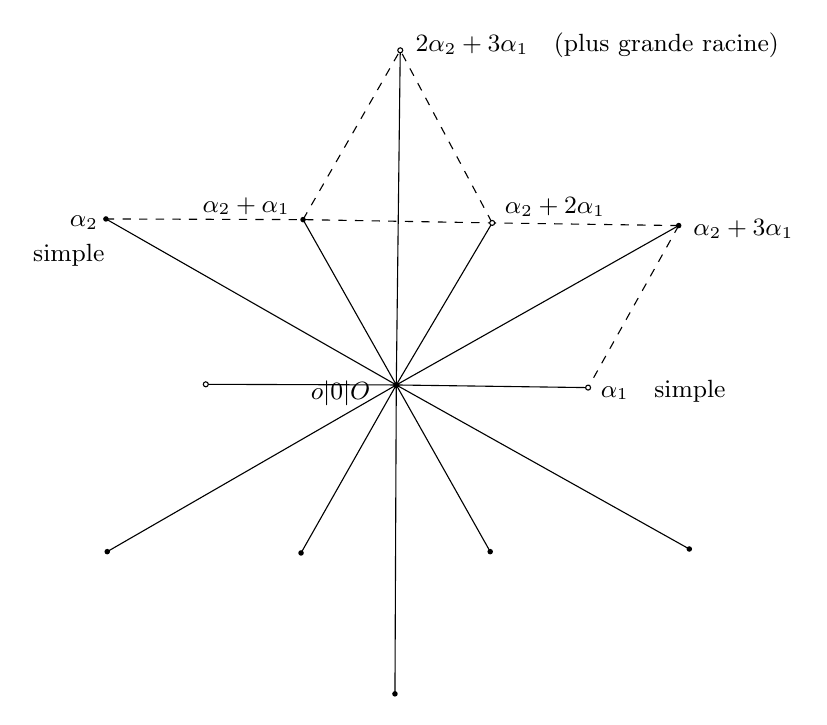
\begin{tikzpicture}[x=.84cm,y=.84cm,every node/.style={inner sep=2pt,font=\small}]
\coordinate (O) at (0,0);
\coordinate (T) at (.06,5.06);
\coordinate (NW) at (-4.39,2.51);
\coordinate (NNW) at (-1.41,2.50);
\coordinate (NNE) at (1.45,2.45);
\coordinate (NE) at (4.27,2.41);
\coordinate (E) at (2.90,-.04);
\coordinate (W) at (-2.88,.01);
\coordinate (SW) at (-4.37,-2.52);
\coordinate (SSW) at (-1.44,-2.54);
\coordinate (S) at (-.02,-4.67);
\coordinate (SSE) at (1.42,-2.52);
\coordinate (SE) at (4.43,-2.48);
\draw[dashed] (NW)--(NNW)--(NNE)--(NE);
\draw[dashed] (NNW)--(T)--(NNE);
\draw[dashed] (NE)--(E);
\draw (O)--(T) (O)--(NW) (O)--(NNW) (O)--(NNE) (O)--(NE) (O)--(E)
      (O)--(W) (O)--(SW) (O)--(SSW) (O)--(S) (O)--(SSE) (O)--(SE);
\fill (NW) circle (1pt) (NNW) circle (1pt) (NE) circle (1pt) (SW) circle (1pt)
      (SSW) circle (1pt) (S) circle (1pt) (SSE) circle (1pt) (SE) circle (1pt);
\draw[fill=white] (T) circle (.9pt) (NNE) circle (.9pt) (E) circle (.9pt) (W) circle (.9pt);
\node[anchor=west] at (.20,5.13) {$\handwritten{2\alpha_2+3\alpha_1}$\quad (plus grande racine)};
\node[anchor=east] at (-4.42,2.46) {$\handwritten{\alpha_2}$};
\node[anchor=north east] at (-4.32,2.22) {simple};
\node[anchor=south east] at (-1.52,2.48) {$\handwritten{\alpha_2+\alpha_1}$};
\node[anchor=south west] at (1.55,2.46) {$\handwritten{\alpha_2+2\alpha_1}$};
\node[anchor=west] at (4.40,2.36) {$\handwritten{\alpha_2+3\alpha_1}$};
\node[anchor=west] at (3.00,-.09) {$\handwritten{\alpha_1}$\quad simple};
\node[anchor=east] at (-.30,-.12) {$\handwritten{\unsure{o|0|O}}$};
\end{tikzpicture}}
\scanpage{61}
% archive sheet number: 60
quitte à passer à une extension finie de $k_0$, $\sigma\leadsto({}^{\sigma}g)^{-1}g$ \deleted{\unsure{ou}} \inserted{inverse de $g^{-1}g^\sigma$}, où $g\in G(\deleted{\unsure{\mathbb C}}k)$ est gén. /$k_0$ \inserted{(point déterminé mod translation par $g_0\in G(k_0)$)}. On trouve alors pour $g^\sigma$ \uline{tt} pt gén de $G(k)$, et par suite $g^\sigma g^{-1}$ peut \deleted{tt} \inserted{\unsure{exhauster|exister|exact}} les valeurs $a$ telles que $\deleted{\unsure{g}}ag$ soit gén /$k_0$, par ex. ttes valeurs telles que que \deleted{\unsure{$(ag)$|$(\sigma)$}} \deleted{\unsure{$ag$}} $a$ soit gén. sur $k_0(g)$.
\deleted{En d'autres \unsure{termes}} Considérons enfin l'hom total $\sigma\longrightarrow\sigma_*$
\diagram{\begin{tikzcd}[ampersand replacement=\&]
\operatorname{Gal}(k/k_0)\arrow[r,"{\deleted{\unsure{\varphi_{\infty}}}\inserted{\unsure{\varphi_v|\phi_v}}}"]\&G(\mathbb A_{\mathbb C})
\end{tikzcd}}

\deleted{\unsure{disons} On \unsure{a envie} de dire que l'image} Considérons le noyau de $\operatorname{Gal}(k/k_0)\unsure{\mathrel{\text{---}}|\longrightarrow}G(\mathbb A_{\unsure{\mathrm{fin}|\mathrm f}})$, qui contient le noyau $\operatorname{Gal}(k/\bar k_0)$ de $\operatorname{Gal}(k/k_0)\unsure{\longrightarrow|\mathrel{\text{---}}}\operatorname{Gal}(k/\bar k_0)$. Ce noyau est envoyé dans $G(\mathbb A_{\mathbb C})$ par $\varphi_{v\infty}$, et l'image est encore dense.
\deleted{De façon plus précise,} \inserted{Il en résulte que} \deleted{\unsure{$\varphi_v$ est}} \deleted{dominant} $\overline{\varphi_v(\operatorname{Gal}(k/k_0)}$ est un sous \unsure{(-groupe)|(-gpe)|(groupe)} ouvert de $G(\mathbb A_{\mathbb C})$.
\margin{(\phantom{o})?}
\scanpage{62}
% archive sheet number: 61
Cette application \unsure{permet|peut} d'écrire, si $w'=\sigma w$
\margin{N.B. c'est ici une petite hyp. restrictive sur $w$\ldots.}
% slanted
\[
M_w^{\mathbb Z}=gM_v^{\mathbb Z}
\]
\[
\begin{aligned}
M_{\sigma w}^{\mathbb Z}&=\dot{\sigma}(M_w^{\mathbb Z})=\dot{\sigma}gM_v^{\mathbb Z}
=\dot{\sigma}g\dot{\sigma}^{-1}(\dot{\sigma}.M_v^{\mathbb Z})
=(\dot{\sigma}g\dot{\sigma}^{-1})\deleted{\unsure{\varphi_v}}\sigma_*^{\deleted{\unsure{g}}}M_v^{\mathbb Z}\\
&=\dot{\sigma}g\dot{\sigma}^{-1}\deleted{\unsure{\varphi_v}}(\sigma_*^{\deleted{\unsure{g}}}g^{-1}\ gM_{\unsure{v|k|w}}^{\mathbb Z}\qquad\text{i.e.}
\end{aligned}
\]
\margin{\unsure{$\dot{t}$|$\dot{\tau}$}}
\[
\left\{\begin{aligned}
M_{\sigma w}^{\mathbb Z}&=\deleted{\unsure{\varphi_w}}(\sigma'_* \deleted{\unsure{)}}M_w^{\mathbb Z}\\
\deleted{\varphi_w(\sigma)=g^{\dot{\sigma}}\varphi_v(\sigma)g^{-1}}&\\
\sigma'_*&=\dot{\sigma}g\dot{\sigma}^{-1}\sigma_*g^{-1}
\end{aligned}\right.
\]
On a donc \inserted{pour $l$ fini}
\[
\sigma'_l=\sigma_l g_l\sigma_l^{-1}\sigma_l g_l^{-1}=\sigma_l
\]
d'où nécessairement
\[
\begin{aligned}
\sigma'_\infty&=\dot{\sigma}_\infty g_\infty\dot{\sigma}_\infty^{-1}\sigma_\infty g_\infty^{-1}\\
&=g_\infty^{\dot{\sigma}_\infty}\sigma_\infty g_\infty^{-1}
\end{aligned}
\]
i.e. on a
\[
\deleted{\varphi_w(\sigma)=g_\infty^{\dot{\sigma}_\infty}\varphi_v(\sigma)g_\infty}
\]
\[
\left\{\begin{aligned}
&\boxed{\varphi_w(\sigma)=g_\infty^{\sigma}\varphi_v(\sigma)g_\infty^{-1}}\\
&\text{pour}\qquad M_w^{\mathbb Z}=gM_v^{\mathbb Z},\qquad g\in G\deleted{\unsure{l}}(M_k(\infty))\\
&\hspace{2cm}\text{i.e. si }w\text{ et }v\text{ sont }\text{\uline{$M$-équivalentes}}
\end{aligned}\right.
\]
